\documentclass[../main.tex]{subfiles}
\graphicspath{{\subfix{../images/}}}
\begin{document}


	All learning processes need {time}. During this time the excitation impulse cycles between the neurons gets chemically fixated on the cortex.
	That leads to the conclusion that {repetition} of the material, as homework and so on, is useful, even necessary. 
	This context sheds a new light on {thinking}: {linking information} to higher, more sophisticated information.
	Learning succeeds best in a stress free, {relaxed atmosphere}, which doesn't exclude healthy performance pressure.

        \begin{figure}[htb]
          \centering
          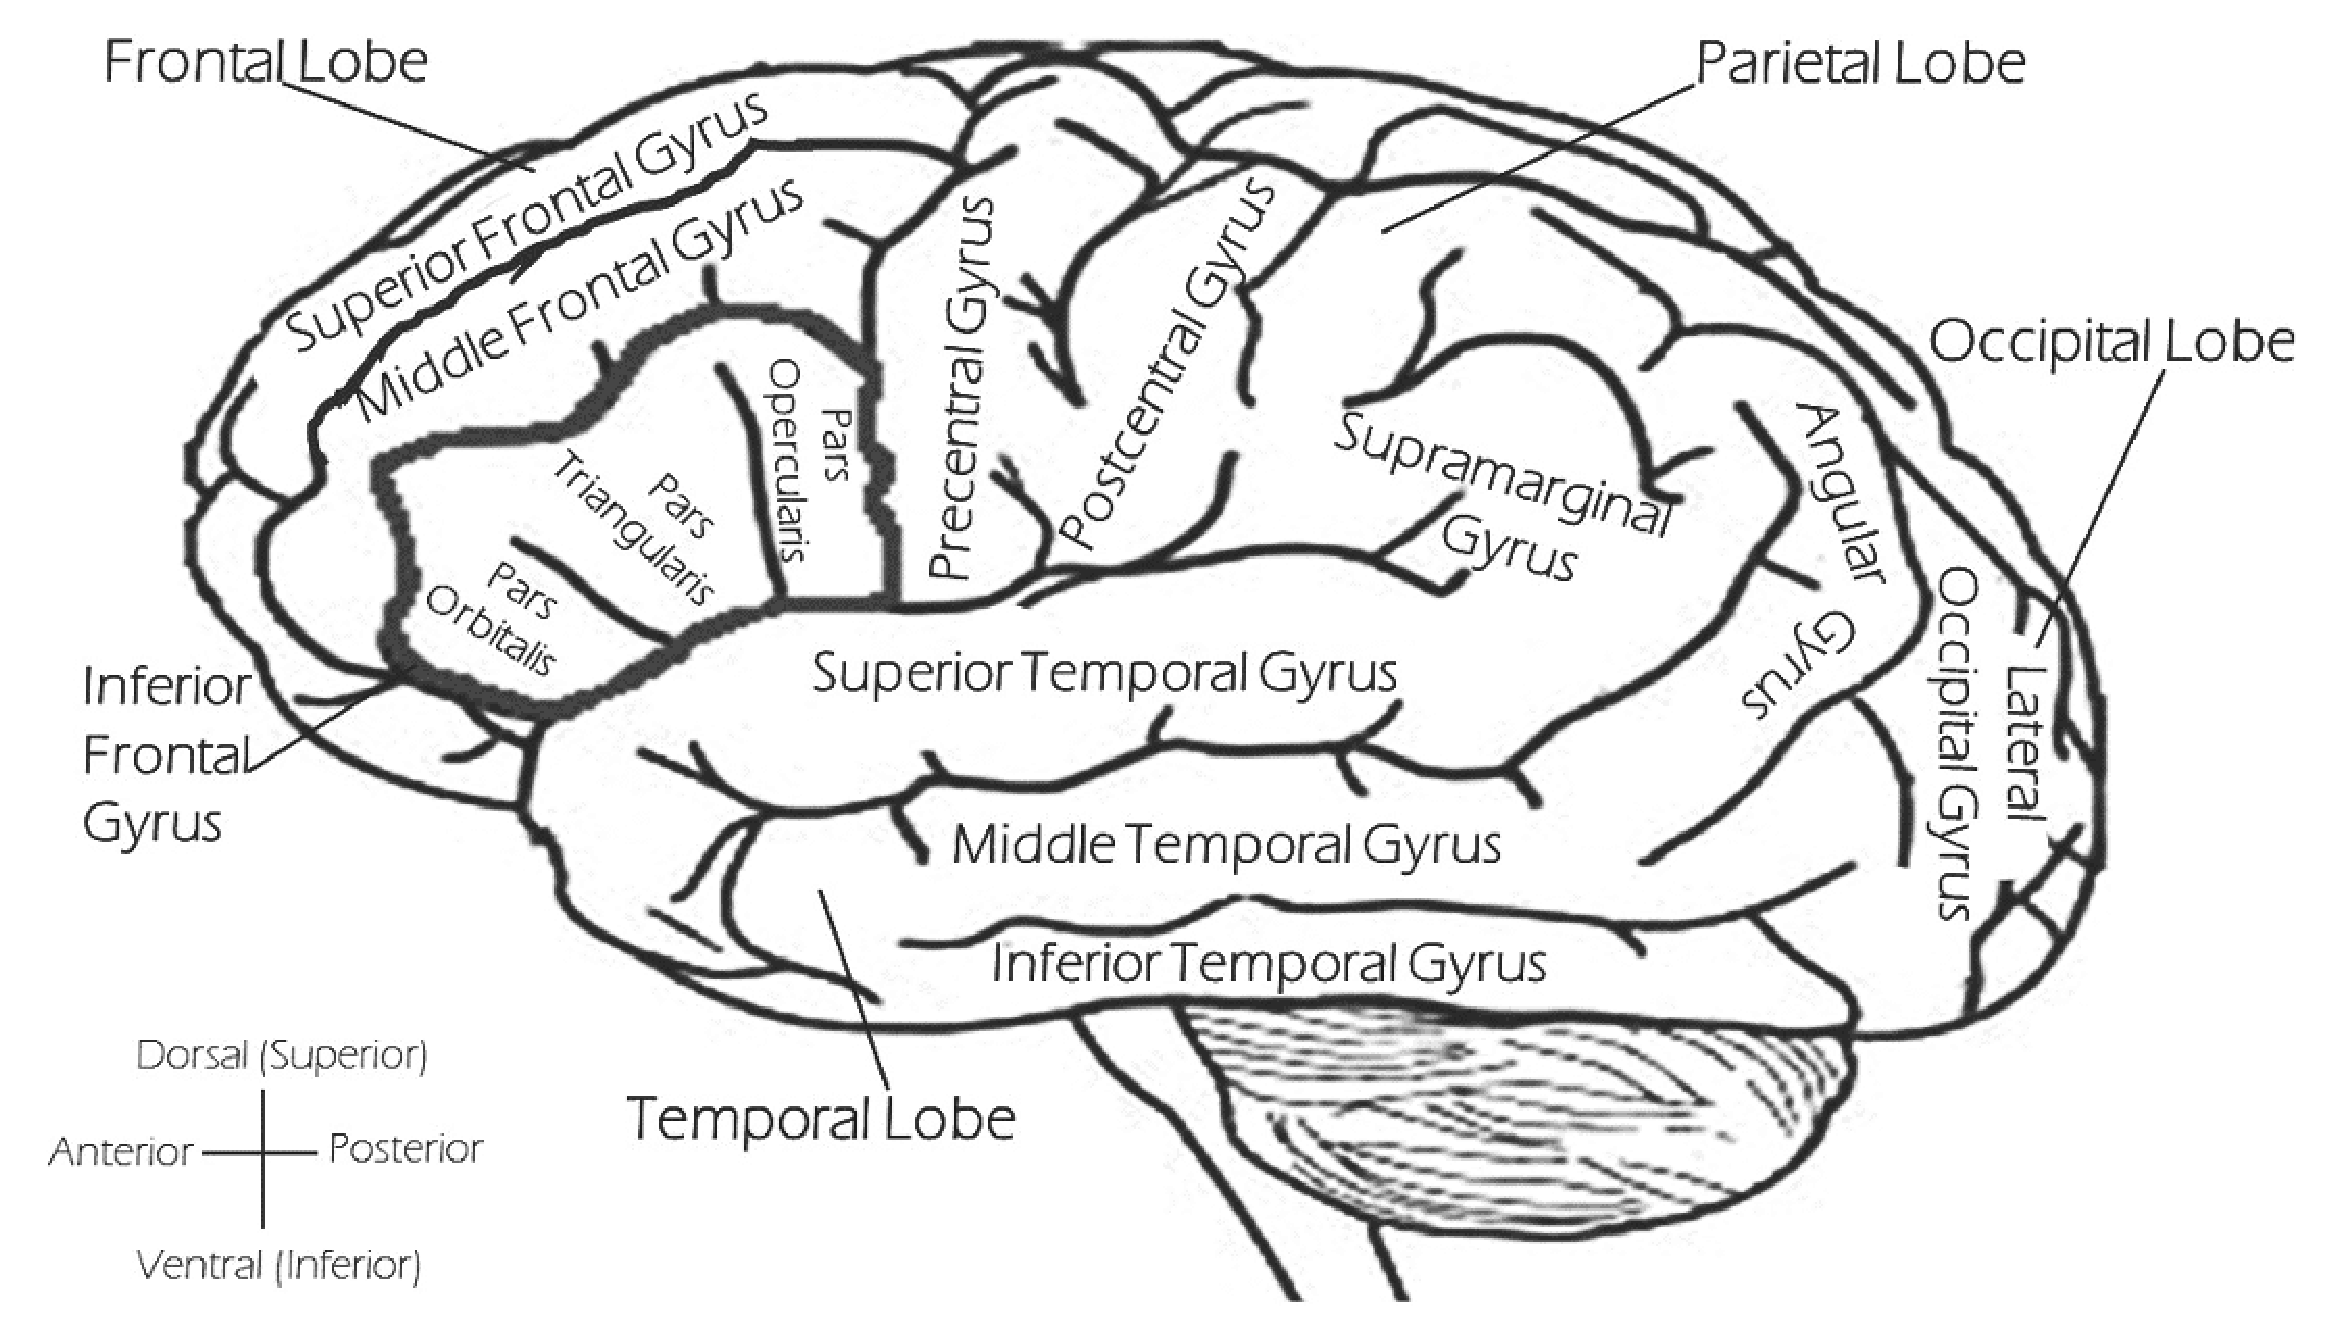
\includegraphics[width=10cm]{brain_labeled.eps}
          \caption{The human brain, labeled~\cite{wclipart}}
        \end{figure}

        The human brain is the most complicated structure know, in average about 44 oz (1245 g) for a female, respectively 48.5 oz (1375 g) for a male brain.\index{brain!weight}
        From a neuro--physiological view all learning and behaviors, all physical processes happen in the brain and get directed by the nervous system.
        The human brain is about triple the weight of the brain of a chimpanzee or gorilla. The Neanderthal had about a more massive brain than modern humans of about 53 oz (1500 g).
        Since the upper paleolithic about 20,000 years ago, there has been a reduction of about 5.3 oz (150 g).
        Out of that reason some scientist assume a permanent reduction of brain mass.\footnote{translated from \textit{Die Evolution des Menschen, Spektrum der Wissenschaft 2003}}

        \setlength\epigraphwidth{.8\textwidth}
        
        \epigraph{Uneducated people are unfortunate in that they do not grasp complex issues, educated people, on the other hand, often do not understand simplicity, which is a far greater misfortune}{\textit{Franz Grillparzer}}
        \setlength\epigraphwidth{.4\textwidth}


\end{document}